\chapter{Analisi concettuale}\label{chap:analisi_concettuale}
\section{L'estrazione dei dati}
\subsection{Requisiti}
Il fine del progetto \`e quello di fornire un servizio portabile che effettui automaticamente lo scraping di dati, in modo massivo, da fonti Social Network. Il software deve garantire un'operativit\`a continua anche a fronte di eventuali problemi relativi al contrasto delle operazioni o inconvenienti tecnici.
Pi\`u informazioni estratte dalle fonti implicano maggiori generazioni di modelli di previsioni ed analisi. Obiettivo operativo del software da produrre \`e la quantit\`a effettiva di dati e la resistenza in campo d'azione.
La portabilit\`a \`e garantita attraverso lo sviluppo di API e la gestione del software in container.
I dettagli tecnici in riferimento alle tecnologie da impiegare sono descritti al Paragrafo \ref{tecnologie_utilizzate}.

Le caratteristiche di un software di scraping ideale riuniscono in questi requisiti:
\begin{itemize}
    \item \textbf{Portabilit\`a}: impiego del software su piattaforme diverse da quella di origine.
    \item \textbf{Interoperabilit\`a}: capacit\`a del software di scambiare informazioni provenienti da pi\`u fonti (es. diversi social network) ed essere in grado di utilizzarle.
    \item \textbf{Resilience to failure}: capacit\`a dell'applicazione di scraping di mantenere l'operativit\`a nonostante eventuali problemi tecnici o azioni di contrasto. \`E importante sviluppare un software resiliente e continuamente aggiornato, osservata l'attenzione da parte dei fornitori dei dati, alla mitigazione dello scraping.
    \item \textbf{Gestione dei dati}: garantire l'uniformit\`a dei formati dei dati, qualora essi provengano da diverse fonti per agevolare la data ingestion.
    \item \textbf{Data ingestion}: processo di trasporto dei dati, necessario per fornire le informazioni ai sistemi di analytics. Gestire un trasporto rapido, veloce e sicuro, consente di apportare migliorie al funzionamento totale del software.
\end{itemize}
\subsection{Infrastruttura}
Per ogni social network oggetto di studio viene sviluppato un connettore che rappresenta idealmente un canale di estrazione ed ingestione dei dati.
Ogni connettore ha caratteristiche differenti a seconda del social individuato come obiettivo. La struttura software della piattaforma target \`e varia e per questo il connettore ed il suo ``motore'' di scraping presentano propriet\`a diverse.
Il punto in comune tra i vari scraper \`e la gestione degli output. Osservato che il canale di immissione dati \`e unico, di conseguenza ogni connettore deve aderire alle policy del sistema di Big Data.
Il singolo data connector ha quindi il compito di estrarre e presentare i dati per il successivo step di analisi.\cite{xu2014information}
Questa attivit\`a rappresenta il fulcro dell'intero progetto e si scontra con le principali problematiche gi\`a descritte come il contrasto tecnico allo scraping e le fattispecie legali.
Il funzionamento tecnico dei connettori individua azioni di estrazione specifica dal target. La ricerca dei dati pu\`o essere effettuata attraverso gli hashtag, i nomi utente, i gruppi e le pagine. Tutto l'output prodotto verr\`a successivamente immesso nel sistema di analisi. 
L'estrazione di un singolo profilo di un utente individua tutta la sua storia sul social, a partire dalla prima informazione pubblicata, fino al giorno in cui avviene l'operazione.

\subsection{Representational state transfer} \label{REST}
Il paradigma REST (representational state transfer) definisce lo stile architetturale per sistemi distribuiti, \`e basato su HTTP ed si basa su quattro principi:
\begin{itemize}
    \item identificazione delle risorse tramite Uniform Resource Identifier (URI);
    \item presenza un'interfaccia uniforme per tutte le risorse;
    \item rappresentazione di risorse e metadati;
    \item presenza di collegamenti ipertestuali.
\end{itemize}
I punti di forza dell'architettura REST si basano sull'assenza di sessione (stateless), sulla scalabilit\`a e sul largo impiego nelle applicazioni web.

L'architettura REST permette di utilizzare i metodi HTTP\footnote{HyperText Transfer Protocol} per la gestione delle risorse.\cite{fielding2000architectural}
In particolare, nel processo di acquisizione dati \`e stato utilizzato il metodo HTTP GET per restituire elenchi e rappresentazioni delle informazioni. Questa azione rappresenta il punto cardine dell'attivit\`a di scraping.


\subsection{Application Programming Interface} \label{API}
Un'interfaccia di programmazione di un'applicazione consiste in un insieme di definizioni, protocolli e procedure messo in atto per favorire l'integrazione e la comunicazione tra diverse applicazioni.
In particolare, un'API \`e detta RESTful quando si attiene ai criteri del paradigma REST citati nel paragrafo \ref{REST}.

Le API REST basano totalmente il loro funzionamento su HTTP, includendone le modalit\`a di richiesta, risposta ed intestazione dei messaggi.\cite{masse2011rest}
\begin{figure}[!htb]
  \begin{center}
  \includesvg[width=400pt]{immagini/api_img.svg}
  \caption{Schema di funzionamento API}
\end{center}
\end{figure}


\subsection{Software container} \label{software_container}
Un software container, lett. ``contenitore di software'', fornisce un ambiente di esecuzione per le applicazioni che condividono un sistema operativo host, codice e librerie con altri container. \cite{syed2015software}
Il vantaggio principale dell'utilizzo dei container \`e la portabilità dello stesso, in quanto pu\`o essere installato ed eseguito su qualsiasi ambiente IT.
Il servizio da implementare è Docker\footnote{\url{https://www.docker.com/}}.
Docker, una piattaforma che garantisce il funzionamento delle applicazioni in qualsiasi ambiente e composta da quattro parti:
\begin{itemize}
    \item \textbf{Docker Engine e Docker Client-Server}: esegue processi secondo l'architettura Client-Server, attraverso un server che opera senza termine (daemon), API Rest per la comunicazione tra i componenti e un client che effettua le richieste;
    \item \textbf{Docker Image}: l'immagine \`e composta da pi\`u strati, a partire dalla base caratterizzata da una distribuzione Linux leggera\footnote{Ubuntu, Fedora, CentOS}. Con la generazione di un Dockerfile e lanciando il comando ``docker build'' viene generata l'immagine;
    \item \textbf{Docker Container}: il container viene generato a partire dall'immagine ed include tutti gli strumenti necessari per avviare ed eseguire l'applicazione.
\end{itemize}
Docker consente di gestire le risorse e standardizzare le applicazioni sviluppate, offrendo soluzioni di distribuzione, prevedendo un eventuale sviluppo di progetto verso l'implementazione di sistemi
distribuiti.\cite{potdar2020performance}
Si riporta lo schema\footnote{Schema tratto da \url{https://docker.com}} della struttura di un container Docker.
\begin{figure}[!htb]
  \begin{center}
  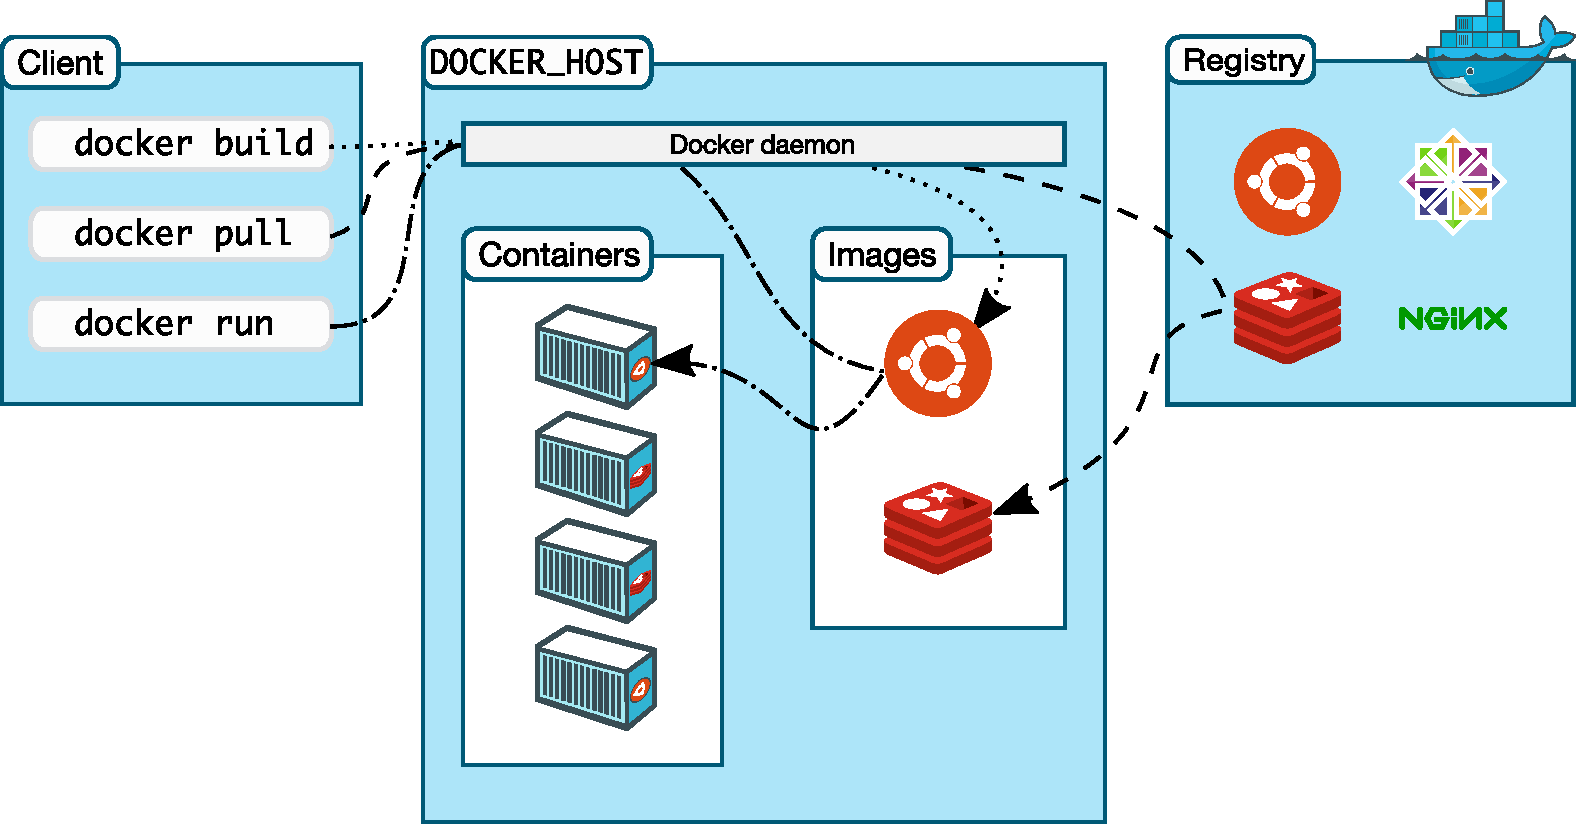
\includegraphics[width=400pt]{immagini/architecture.pdf}
  \caption{Struttura di un container Docker}
\end{center}
\end{figure}
\newpage

\subsection{Cookies} \label{cookieitem}
I cookies rappresentano dei piccoli blocchi di dati, generati lato server e memorizzati sul client, in grado di espletare varie funzioni.
Nella loro configurazione \`e possibile definire diversi attributi a seconda dello scopo di utilizzo degli stessi.

La diversificazione nel loro impiego, identifica diverse tipologie di cookies: 
\begin{itemize}
    \item \textbf{Cookie di sessione}: vengono generati nel momento in cui l'utente effettua operazioni di navigazione web, scadono una volta che viene chiuso il browser.
    \item \textbf{Cookie persistenti}: basano il loro funzionamento su uno specifico arco temporale. In particolare vengono memorizzati lato client e trasmessi nel caso in cui si ha la necessit\`a del loro impiego in un determinato sito web. Una volta terminato il periodo di validit\`a scadono e devono essere generati nuovamente.
    Questa tipologia di cookie viene adottata dai siti web in cui \`e presente un form di autenticazione, mantenendo in questo modo il login.
    \item \textbf{Cookie di terze parti}: tracciano l'attivit\`a dell'utente attraverso la navigazione nei siti web. Vengono impiegati in ambito pubblicitario e generano il collegamento a server differenti da quello in cui si sta fruendo un determinato servizio, per recuperare informazioni memorizzate durante tutta la sessione di navigazione. 
\end{itemize}
L'utilizzo dei cookie, impone una maggiore gestione della sicurezza, soprattutto nella memorizzazione dati relativi a sessioni di login.\cite{kristol2000http}
I cookie di tipologia persistente, vengono impiegati durante l'accesso ai social network;  il salvataggio di questi dati, permette di effettuare login ai servizi, senza l'utilizzo di credenziali.

\subsection{L'ingestione dei dati}
Per Data Ingestion si intende il processo di raccolta dei dati raw (grezzi) dalla loro sorgente e del trasporto e la centralizzazione verso il sistema target.\cite{meehan2017data}

Viene definito anche ETL (Extract/Transform/Load) ovvero estrazione, trasformazione e caricamento. Le tre fasi funzionali assolvono i seguenti compiti:
\begin{itemize}
    \item \textbf{Estrazione}: la prima fase attua le tecniche definite al Capitolo \ref{chap:stato_arte}. Le soluzioni adottate per l'elusione dei controlli e la mitigazione del contrasto saranno dettagliate al Paragrafo \ref{contrasto_scraping}. 
    \item \textbf{Trasformazione}: la seconda fase  si occupa del controllo e del data cleaning, ovvero il processo in grado di garantire l'affidabilit\`a dei dati, anche trasformandoli in formati idoeni al loro utilizzo. Nel caso del progetto di tesi \`e stato scelto il formato JSON, dettagliato al Paragrafo \ref{formato dati}.
    \item \textbf{Caricamento}: la terza e ultima ultima fase rappresenta il caricamento dei dati nel sistema di Big Data Analytics. La gestione di questo step \`e garantita attraverso l'omogeneit\`a negli output e nelle tecnologie richieste dal target per ogni connettore.
\end{itemize}


\subsection{Big Data Analytics}
Con il termine Big Data si definisce un sistema avente tre attributi: grande volume di dati, variet\`a e velocit\`a. 
Il volume rappresenta l'attributo principale, seguito dall'eterogeneità e dalla frequenza di generazione e rilascio dei dati.

L'applicazione del termine ``Big Data Analytics'' comprende tecniche avanzate di analisi dei dati su set di Big Data.\cite{russom2011big}
L'analisi dei dati si distingue a seconda degli strumenti e dei modelli di gestione in tre tipologie:
\begin{itemize}
    \item \textbf{Analisi descrittiva}: descrizione storica e confronto dei dati presenti. Tecnica da impiegare per la catalogazione delle informazioni attuali e passate. 
    \item \textbf{Analisi predittiva}: applicazione di modelli predittivi sui dati, in grado di estrarre e prevedere casi futuri. 
    \item \textbf{Analisi prescrittiva}: propone soluzione automatizzate ed implicazioni di azioni in corso sui dati.
\end{itemize}
L'insieme dei tre modelli di analisi sono applicabili per lo scopo del progetto ed il conseguente studio delle informazioni pubbliche estratte dai social.
\section{Soluzioni al contrasto dello scraping}\label{contrasto_scraping}
\subsection{Generalit\`a}
Le metodologie attuate dalle piattaforme social per contrastare l'attivit\`a di scraping sono state elencate e descritte al Paragrafo \ref{metodi_contrasto}. Si presentano di seguito soluzioni ideali per garantire il funzionamento di un'applicazione resiliente ed in grado di offrire l'estrazione della maggiore quantit\`a di dati.

%%%%%%%%%%%%%%%%%%%%%%%%%%%%%%%%%%%%%%%%%%%%%%%%%%%%%
%aggiungere

\subsection{Gestione degli account} \label{account}
I social network, per la normale attivit\`a sulle loro piattaforme, obbligano ad effettuare la registrazione ed il conseguente login. Le possibilit\`a di accesso ai servizi senza alcuna tipologia di autenticazione sono molto limitate e non giovano in alcun modo ad una completa estrazione dati. Da ci\`o ne consegue la necessit\`a di autenticarsi ai servizi e la creazione di un pool di account. 
L'idoneit\`a di un account risulta essere oggetto di attenzione dai servizi web dei social. Le soluzioni di sicurezza ``anti-bot''\footnote{Con il termine ``bot'' si fa riferimento ad un servizio che compie azioni in modo automatico} sono in grado di individuare la generazione di utenti falsi, definiti ``fake accounts'' promuovendo ed attuando il loro ban.
\subsection{Rotazione dei Cookies}\label{cookie rotation}
Una volta avuta la disponibilit\`a di un numero cospicuo di account validi, si procede con l'azione di login e la successiva estrazione dei cookie, per ogni utenza.
L'estrazione dei cookie pu\`o avvenire attraverso l'accesso diretto dal tool di scraping, oppure tramite lo sviluppo di azioni in funzione di applicazioni di browser automation. 
La seconda opzione risulta essere maggiormente indicata, soprattutto in visione della scadenza di validit\`a temporale dei singoli cookie, che rende obbligatoria la ripetizione del login. 

Un recupero della sessione automatico e il conseguente aggiornamento dei cookie consente la validit\`a continua degli stessi.
Una soluzione implementativa idonea all'elusione del controllo sullo scraping \`e l'introduzione, dopo aver memorizzato tutti i cookie validi degli account, di un sistema di rotazione random sulla selezione ed impiego del cookie appartenente ad un determinato utente.
Questa operazione consente di diversificare gli accessi automatici al social, limitando fortemente la probabilit\`a di ban di un account, osservato che lo stesso verr\`a impiegato per una singola operazione alla volta e successivamente sostituito da un altro nell'elenco, diminuendo cos\`i l'esposizione del singolo.

Ne consegue che un maggior numero di account validi disponibili per l'accesso al social network, consente una massimizzazione dell'elusione al controllo sul singolo utente e la sua attivit\`a.
Avendo pi\`u cookie in grado di essere selezionati dalla funzione random, viene aumentata l'operativit\`a continua, in senso temporale, dell'estrazione dei dati.  

\begin{figure}[!htb]
  \begin{center}
  \includesvg[width=425pt]{immagini/cookie_rotation.svg}
  \caption{Cookie Rotation}
\end{center}
\end{figure}
\newpage

\subsection{Latenza}
Il contrasto alle soluzioni anti-scraping richiede anche un tempo operativo pi\`u dilatato. Si rende necessaria l'aggiunta di latenza tra le operazioni in termini di secondi o minuti, garantendo un profilo di attivit\`a non sospettoso.
L'aggiunta di tempo d'attesa tra le operazioni consente la simulazione dell'attivit\`a umana sulla piattaforma web, non dimostrando l'automaticit\`a e la velocit\`a tipica dei bot.
Un'idea implementativa \`e l'introduzione di attesa random nell'ordine dei minuti. Alcuni tool di scraping prevedono automaticamente una funzione di salvaguardia dell'account, bloccando le richieste ed azionando un'attesa a seconda dell'onerosit\`a dell'attivit\`a da svolgere.
Considerato che l'obiettivo del progetto \`e la garanzia operativa senza l'effettiva necessit\`a di velocit\`a nella produzione dei dati, il ritardo tra le azioni non vincola l'impiego del software da produrre.

\subsection{User Agent}
Lo user agent identifica un campo del protocollo HTTP in cui vengono dichiarate delle informazioni relative al dispositivo che si connette al server ed il browser utilizzato.
Un esempio di user agent valido per la connessione ad Instagram e relativo ad un dispositivo mobile iOS \`e il seguente:
\begin{center}
    Mozilla/5.0 (iPhone; CPU iPhone OS 15\_5 like Mac OS X) AppleWebKit/605.1.15 (KHTML, like Gecko) Mobile/15E148 Instagram 244.0.0.12.112 (iPhone12,1; iOS 15\_5; en\_US; en-US; scale=2.00; 828x1792; 383361019)
\end{center}
Nell'atto dello scraping \`e importante definire user agent idonei ed approvati dal servizio target in quanto lo stesso pu\`o effettuare specifici controlli e non accettare le richieste provenienti da user agent non presenti in ``white-list''\footnote{Si fa riferimento all'elenco degli user agent accettati dal servizio.}.
\subsection{Indirizzi IP}\label{ip_rotation}
I sistemi anti-scraping pongono particolare attenzione agli indirizzi IP dai quali provengono le richieste. Come introdotto al Paragrafo \ref{metodi_contrasto}, viene attuato un controllo sulla affidabilit\`a dell'indirizzo da cui si \`e connesso un determinato utente. Nel caso in cui venissero rilevate delle azioni ``insolite'' o massive, si procede con il ban temporaneo o permanente, a seconda delle policy previste dal servizio.

Un'idea implementativa \`e l'utilizzo di un pool di indirizzi IP da proxy condivisi. L'introduzione di una ``ip-rotation'' randomica, seguendo quanto progettato per la cookie-rotation (Paragrafo \ref{cookie rotation}), pu\`o diminuire il numero di ban e garantire un maggiore impiego delle utenze a disposizione.

Si riporta uno schema per il funzionamento di ``ip-rotation''.
\begin{figure}[!htb]
  \begin{center}
  \includesvg[width=425pt]{immagini/ip_rotation.svg}
  \caption{IP Rotation}
\end{center}
\end{figure}
\subsection{Sistemi distribuiti}\label{sistemi_distribuiti}
Un sistema distribuito \`e un insieme di processi indipendenti ed interconnessi che cooperano per la condivisione di risorse. \cite{tanenbaum2007sistemi}

Le caratteristiche dei sistemi distribuiti sono:
\begin{itemize}
    \item \textbf{Openess}: possibilit\`a di estendere, in termini di risorse, un sistema.
    \item \textbf{Concurrency}: presenza di pi\`u processi coesistenti su un'unica risorsa.
    \item \textbf{Scalability}: capacit\`a del sistema di aumentare ed adattarsi all'aumento dimensionale del lavoro da compiere senza alterare la funzionalit\`a.
    \item \textbf{Fault tolerance}: tollerenza del sistema al guasto.
\end{itemize}

%%%%%%%%%%%%%%%%%%%%%%%%%%%%%%%%%%%%%%%%%%%%%%%%%%%%%
%continuare
L'implementazione della distribuzione su un'applicazione di scraping consente di ottenere molteplici vantaggi oltre a quelli propri dei sistemi distribuiti.
Pu\`o essere identificata come una soluzione generalizzata al contrasto dello scraping, in quanto consente di aggiungere funzionalit\`a utili all'elusione dei controlli.
La funzionalit\`a di un sistema distribuito per lo scraping necessita della presenza di un controller in grado di inviare comandi ai singoli nodi e ricevere risposte in termini di dati estratti dai singoli scraper-bot.
La comunicazione tra controller e singoli bot pu\`o avvenire tramite Remote Procedure Call (RPC) \footnote{Indica una procedura avviata su dispositivo diverso da quello sul quale viene eseguito un programma.}
Si presentano di seguito gli schemi di funzionamento e comunicazione delle varie parti in azione durante lo svolgimento di un'attivit\`a di scraping distribuita.

%%%%%%aggiungere info su sistemi distribuiti

%Idea di scraping distribuito con schema 
\begin{figure}[!htb]
  \begin{center}
  \includesvg[width=400pt]{immagini/distributed_scraper.svg}
  \caption{Schema di un'applicazione di scraping distribuita}
\end{center}
\end{figure}

\begin{figure}[!htb]
  \begin{center}
  \includesvg[width=400pt]{immagini/bot_controller.svg}
  \caption{Schema di comunicazione controller-bot}
\end{center}
\end{figure}
%\clearpage
\newpage
\section{Output}
\subsection{Gestione dei dati estratti}
I dati in output devono essere uniformi e pronti all'ingestione in un sistema di analisi. Per garantire l'uniformit\`a si devono individuare formati e tipi di dato uguali, a fronte dell'estrema eterogeneit\`a dei dati raccolti. 
Un esempio \`e l'introduzione dell'utilizzo di UUID (Universally Unique Identifier) per la denominazione dei file e la compressione delle cartelle in formato zip per la riduzione dello spazio di memoria occupato. UUID rappresenta un identificativo univoco universale composto da 128 bite rappresentato da caratteri esadecimali divisi in gruppi.
Si fa presente che i dati effettivamente estratti restano in formati direttamente fruibili quali JSON, JPEG e MP4. L'impiego di UUID e zip ha come obiettivo la sola modifica della denominazione e della dimensione dei file per la loro successiva ingestione ed analisi come Big Data.

Diversi tool offrono la possibilit\`a di individuare file gi\`a presenti in locale, frutto di estrazioni precedenti, evitando di effettuare un nuovo download. Questa funziona viene adottata anche per individuare eventuali cambiamenti ``storici'' nell'account target: nel caso in cui un elemento gi\`a estratto in passato non venga pi\`u selezionato e scaricato, si deduce automaticamente la presenza di un'azione di cancellazione dello stesso dalla piattaforma social.

L'analisi comportamentale del software rispetto a cambiamenti storici nell'output garantisce un elevato numero di informazioni aggiuntive che vanno ad ampliare i metadati gi\`a frutto di estrazione. Le stesse, combinate con il resto, garantiscono una continuit\`a informativa nell'atto dell'ingestione dei dati nel sistema di Big Data Analytics.

Si riporta di seguito uno schema di gestione dei dati di output provenienti dal software di scraping.

\begin{figure}[!htb]
  \begin{center}
  \includesvg[width=400pt]{immagini/output.svg}
  \caption{Schema di gestione dei dati per l'ingestione}
\end{center}
\end{figure}
\newpage
